\documentclass[11pt,a4paper]{article}
%PKG
\usepackage[utf8]{inputenc}
\usepackage[english]{babel}
\usepackage{amsmath}
\usepackage{amsfonts}
\usepackage{amssymb}
\usepackage{hyperref}
\usepackage{textcomp}
\usepackage{graphicx}
\usepackage{listings}
\usepackage{verbatim}
\usepackage{subfig}
\usepackage[a4paper, total={6in, 9in}]{geometry}
\usepackage[font=small,labelfont=bf, textfont=sl]{caption}
\usepackage{multicol}

%Graphics
\graphicspath{{./media/}}

%FUNCTIONS
\newcommand{\centerFigure}[2]{
\begin{figure}[ht]	
%Image: #1
\centering
\includegraphics[width=10cm]{#1}
\caption{#2}
\end{figure}
}
%DOCUMENT
\begin{document}
\pagestyle{plain}
\author{Jeanne, Axel \and Arias, Monica}
\title{Supervised Mobile Manipulator}
\maketitle
\begin{abstract}
Teleoperation in robotics was the first widespread application of robots. 
It was mainly used in applications involving operations in hazardous area for humans (space, 
radioactive, high temperatures, etc.)

The goal of the Supervised Mobile Manipulator (SMM) project is to build a robotic system used for
teleoperation from a remote area. It is using one robot performing a task and another robot as 
``assistant" to provide help to the operator when performing manipulation actions. To enable a single operator to control both robots some cooperative behaviours were implemented.

In this paper we will present the platforms and tools we have used, then we will present the developed 
work on the robotics system and finally present our experiences and results.
\end{abstract}
\clearpage

\tableofcontents

\clearpage
\section{Theoretical content}
\subsection{Advantages of cooperative system}
In most cases, the operator performing a task remotely only has a single point of view: the
one of the embedded camera. In multiple different systems, this can
lead to inconvenient situations where the operator is performing a task with a sub-optimal
vision of the situation.

One solution to this problem could be to add an animate vision system \cite{Ballard1991}
but this kind of solution vastly increases the complexity of the system since the whole vision system
has to be actuated. Another solution could be to increase the number of cameras on the robot.
This solution increases the robot payload and is actually not very convenient for the user
since more video streams now have to be monitored while performing the task. The solution we chose is to add an external robot to provide a ``supervisor" vision of the acting robot. This solution adds many different  advantages:

\begin{enumerate}
\item The supervisor can provide vision from different angles while the action robot is static
\item The supervisor can scout ahead of the action robot to ensure safety
\item The supervisor behaviours can be automated to unload the operator's attention
\end{enumerate}


\subsection{Problem statement}
The Supervised Mobile Manipulator Project (SMM) goal is to develop a cooperative robotics
system which can be used in hazardous areas. It uses two platforms: 

\begin{itemize}
\item An action platform which perform the physical operation
\item A supervisor platform which keeps an overview of the situation
\end{itemize}

A diagram of the system can be seen in Figure 1.

To deliver a fully applicable solution, a GUI (Graphical User Interface) is provided in
order to see what the system is doing in real time.

\centerFigure{teleopSystem.png}{The tele-operated robotic system}


\subsection{Tools used}
\subsubsection{Git}
To deliver a complete solution, a lot of software development was required. In order to keep
the code maintained and keep track of changes in code; we used \href{https://git-scm.com/}{git} as a version control system
 (VCS). The repository for the developed nodes and the GUI can be found at \verb!rescuer_project!  \footnote{https://github.com/axilos22/rescuer\_project} and for the simulation environment at \verb!rescuer_sim!\footnote{https://github.com/MonicaArias/rescuer\_sim}.

\subsubsection{ROS}
\href{http://www.ros.org}{ROS} stands for Robotic Operating System, although it is not technically an OS. ROS is a middleware that provides an easy to use communication platform for different software and hardware elements. ROS was a very useful tool to implement cooperation in our system, particularly the network communication among robots.

\subsubsection{Gmapping}
The \href{http://wiki.ros.org/gmapping}{Gmapping} ROS package is an implementation of the Simultanous Localization and Mapping (SLAM) algorithm. It builds a grid map from a laser scan, and localizes the robot from odometry data and features extracted from the environment.

\subsubsection{Navigation Stack}
The \href{http://wiki.ros.org/navigation}{Navigation} ROS package enables a mobile robot to avoid obstacles in the environment (based on sensor readings), make a plan to reach a goal and produces appropriate velocities to get there. It accomplishes this through two separate implementations. 

First it builds a global costmap of the perceived environment, and builds a global path from the current position to the goal based on Djisktra's algorithm, obtaining the lowest cost path. This part is platform independent. 

Secondly it builds a local costmap, taking into account close obstacles and the global path, and sends the command velocities to the platform. The local planner is  platform dependant, and has to be tuned for optimal performance.

\subsubsection{Tum Ardrone}
The \href{http://wiki.ros.org/tum_ardrone}{Tum Ardrone} ROS package allows us to control the AR Drone at a higher level. It implements three nodes: 

\begin{itemize}
\item State Estimation: Provides an estimate of the drone's position from the navigation data sent by the drone, the velocity commands and the tracking of key points in the front camera image. It uses Extended Kalman Filter (EKF) and Parallel Tracking and Mapping (PTAM) simultaneously for more accurate prediction.

\item Autopilot: Provides a PID position controller for the AR Drone. The gains are already tuned correctly, but an aggressiveness parameter can be set to modify the response time.

\item Graphical User Interface: Monitors and controls the State Estimation and Autopilot nodes.

\end{itemize}

\subsubsection{Gazebo}
Gazebo is a well known and widely used simulator with a robust physics engine. 
Robot platforms like the AR Drone are already implemented, and new robots can be added using a URDF description. It also counts with different plugins  for robot, sensor, and environmental control. 
subsubsection{Qt}
Qt is a well known GUI library. Is is used a large variety of applications from mobile phone interfaces to advanced customized programs. Qt is so popular that a module for ROS was
created called rqt (ROS Qt).


\subsection{Mobile manipulator}


The mobile manipulator used consists of the Guardian platform as mobile base, and the WAM\texttrademark  arm with the BarretHand\texttrademark  as manipulator (Figure \ref{fig:gwam}). The Guardian is a Robotnik modular platform with high mobility and speed, small enough to be transported in a conventional car boot. 

Barret Techonology developed both the WAM\texttrademark arm, with 7 degrees of freedom, and the BarretHand\texttrademark  with three fingers, each one with one degree of freedom to stay at a fixed closed position, and an additional degree of freedom which defines the aperture of the three fingers.

Our mobile base was equipped with a Microsoft Kinect, which uses an infrared sensor and adaptive depth detection technology. Having such information is very interesting for 
navigation
purposes since the relative distance to object is easily accessible.

\begin{figure}[ht]	
\centering
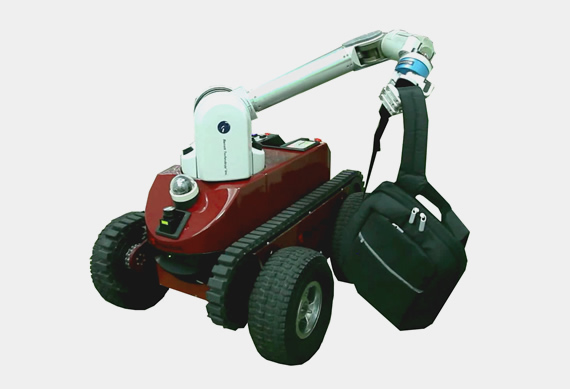
\includegraphics[height=4cm]{gwam1.jpg}
\caption{Guardian with Barret WAM arm}
\label{fig:gwam}
\end{figure}

\subsection{Quadrotor}

The quadrotor used is a Parrot\textcopyright AR Drone v2\texttrademark , a 4 propellers
drone which has a ROS compatible driver. It is also equipped with two cameras: one in front
and another in the bottom. The bottom camera can be used for visual tracking and the drone
has an on-board tracking system, allowing a decent tracking without latency issues.

\begin{figure}[ht]	
\centering
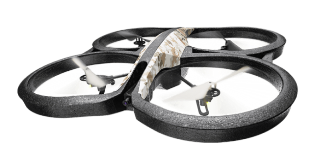
\includegraphics[height=3.7cm]{arDroneGpsEdition.png}
\caption{AR Drone v2}
\end{figure}

Additionally, some ROS libraries have been created to be compatible with the drone; we used
one of them called \href{"http://wiki.ros.org/tum_ardrone"}{"tum\_ardrone"} in parallel with
the driver package: \href{"https://github.com/AutonomyLab/ardrone_autonomy"}
{"ardrone\_autonomy"}.

\subsection{Cooperative behaviours}
As the two robots have to cooperate to perform their common goal, it was required to implement different cooperative behaviours
on the system. During the conceptualization of the project we established different
 behaviours that the system should be able to manage: decoupled, coupled and supervisor mode. Figure \ref{fig:Coop} displays a diagram of these behaviours.

\begin{figure}[ht]	
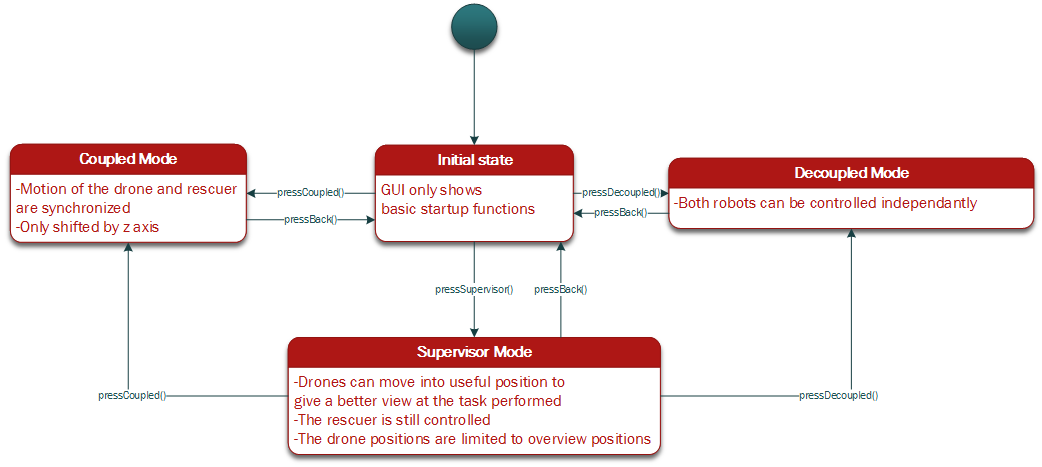
\includegraphics[height=7cm]{cooperativeModes.png}
\caption{Cooperative behaviours states map}
\label{fig:Coop}
\end{figure}

\subsubsection{Default mode}
The default mode is the one in which the system start. No particular behaviour is expected but the two
robots should establish connection and start exchanging their respective localization and status data.

\subsubsection{Coupled mode}
In this mode the two robots communicate to reach a user defined goal. The mobile base handles the path planning and navigation, and the drone follows. The drone tracks the mobile base by requesting the mobile base location. From this point forward, if the mobile base moves, the drone remains on top and moves along with it.

\subsubsection{Decoupled mode}
This mode is the same as default mode in terms of behaviour. The only difference is that the default mode
is not accessed any more after start-up. When the system enters the decoupled mode, the two robots movements
are decoupled and can be separately controlled, either by tele-operation or any other method.

\subsubsection{Supervisor mode}
The supervisor mode is a semi-operated mode. In this mode, the drone will adopt a set of pre-defined
positions around the mobile base. For
instance adopting a lateral camera position while the robot is grasping an object. This would
allow the operator to have a real-time visual feedback on the action. 



Additional behaviours can be added into the supervisor mode to be even more effective, in the case of navigation, the drone could move 
among a semi-circle (or full circle) around the mobile platform, allowing the 
operator to have better awareness of the situation (Figure \ref{fig:assist}). Another behaviour
could be ``forward scouting" allowing the drone to explore the area before engaging the 
mobile base.

\begin{figure}[ht]	
\centering
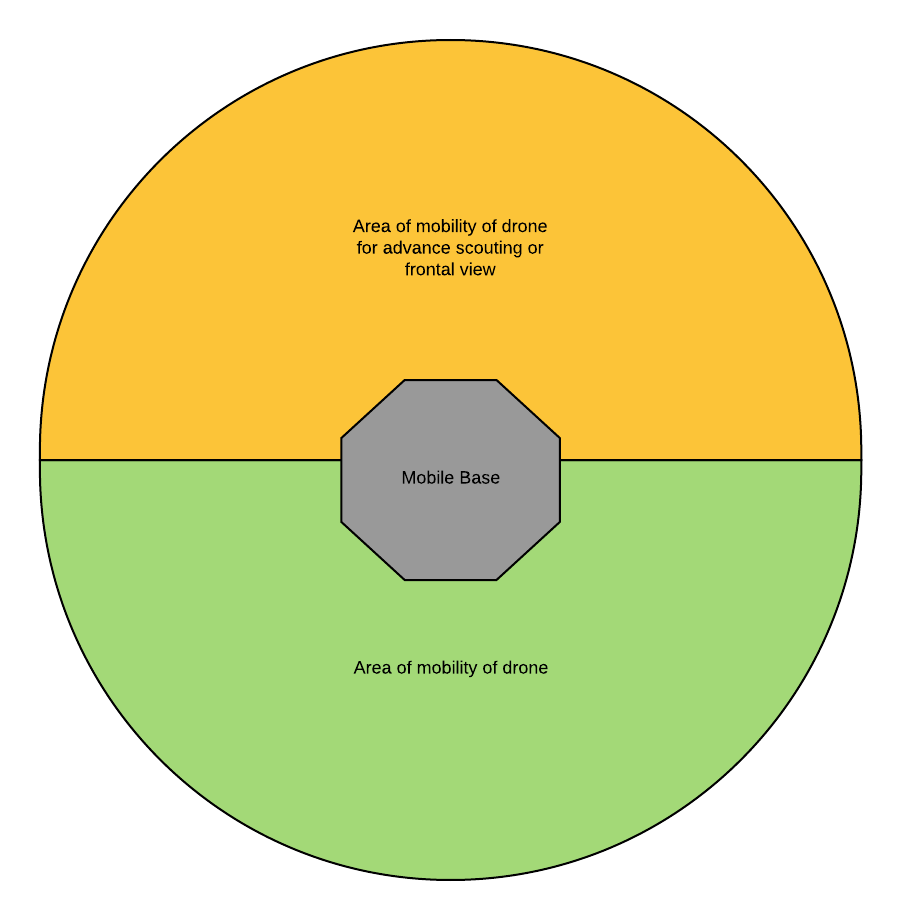
\includegraphics[height=8cm]{assistanceBehavior.png}
\caption{Map of the assistance behaviour}
\label{fig:assist}
\end{figure}

\clearpage

\section{Work achieved}

\subsection{Simulator implementation}
In order to debug and test the cooperative behaviours we built a simulation of the whole system in Gazebo. 
We used the following ROS packages to simulate the robots:

\begin{itemize}
	\item \verb!guardian_sim! \footnote{https://github.com/RobotnikAutomation/guardian\_sim} - For the Guardian and the WAM\texttrademark arm
	
	\item  \verb!barret_hand_sim!  \footnote{https://github.com/RobotnikAutomation/barrett\_hand\_sim} 
	and \verb!barret_hand_common! \footnote{https://github.com/RobotnikAutomation/barrett\_hand\_common}
	- For the BarretHand\texttrademark
	
	\item  \verb!tum_sim! \footnote{https://github.com/tum-vision/tum\_simulator.git}  - For the AR Drone
\end{itemize}

The Guardian and the WAM\texttrademark arm's simulator packages were developed for the Hydro version of ROS, one previous to the one we are using (Indigo). It was required to do some slight modifications to the URDF description files to make them compatible with our system. The files for the Guardian are located in the \verb!guardian_description! subpackage and for the WAM arm in the \verb!robotnik_wam_description! subpackage of \verb!guardian_sim!. For each position controller (declared as transmission) we had to add the hardware interface element to the joint name definition, like shown in Figure \ref{fig:urdf}.

\begin{figure}[ht]	
	\centering
	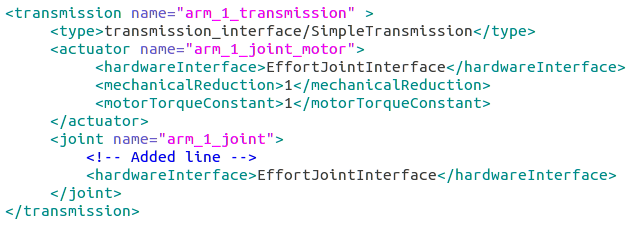
\includegraphics[width=12cm]{arm_trans.png}
	\caption{Modification of the ``wam\_guardian.urdf.xacro'' file of the guardian\_sim package}
	\label{fig:urdf}
\end{figure}



An additional modification was that, in the files provided by Robotnik to simulate the Guardian, the gravity element was at $-1$ $ m/s^2$ to allow the platform to move in the simulated world. To increase the gravity value to the real $-9.8$ $ m/s^2$ we had to reduce the defined weight of the main body from 95 kg to 15 kg. We obtained a good translational movement but it was quite challenging to rotate the platform, therefore the navigation stack took longer to reach the desired orientation. 


For controlling each robot we used gazebo plugins. The skid steer drive controller  allowed us to control the Guardian by sending a velocity message. We declared it in the 
``gwam.gazebo'' file of the \verb!guardian_description! package, shown in Figure \ref{fig:gcontrol}. The four joints representing the wheels were declared in the ``guardian\_wam.urdf.xacro'' file. By setting the \textit{broadcastTF} element to \textbf{True} the plugin is supposed to broadcast the position of the robot  measured by odometry as the \textit{odom} frame, needed for the navigation stack.  In our implementation, with ROS Indigo and Gazebo 2.1, this feature was not working, therefore it was necessary to modify the default from \textbf{False} to \textbf{True} in the source file, obtained from the \verb!gazebo_ros_pkgs! \footnote{https://github.com/ros-simulation/gazebo\_ros\_pkgs/tree/indigo-devel} package.



\begin{figure}[ht]	
	\centering
	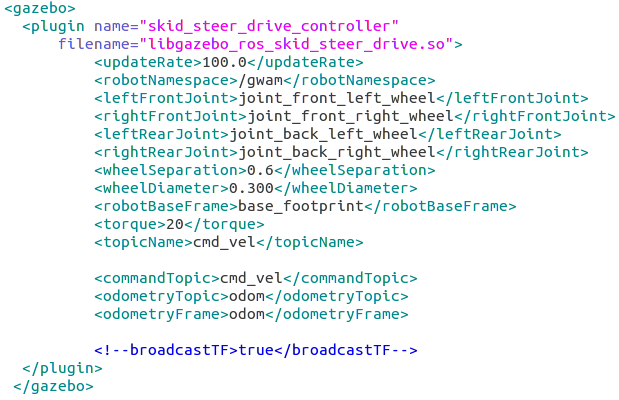
\includegraphics[width=12cm]{gwam_gazebo.png}
	\caption{Skid steer drive controller for the Guardian}
	\label{fig:gcontrol}
\end{figure}

The control of the joints for the arm and the hand did not need to be declared in the description files. Instead they were added to the ``gwam\_control.yaml'' file located at the \verb!guardian_control! subpackage, and loaded in the launch file. In Figure \ref{fig:armcontrol} we can see an example of the position control for the first joint of the arm (of seven) and the first joint of the hand (of four). With these controllers we can set the position of each joint by publishing a message once and the controller will maintain the joint at the right position.

\begin{figure}[ht]	
	\centering
	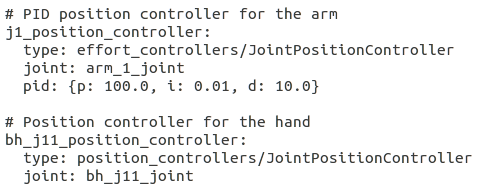
\includegraphics[width=9cm]{arm_yaml.png}
	\caption{Examples of position controllers for the WAM arm and the BarretHand}
	\label{fig:armcontrol}
\end{figure}

Once we had full control of the mobile manipulator, we noticed that when the mobile manipulator attempted to grasp an object, it slipped. This can be solved by fine tuning the material properties of the object and the gripper, or by using the gazebo grasp plugin from the \verb!gazebo-pkgs!\footnote{https://github.com/JenniferBuehler/gazebo-pkgs} package. The plugin detects when two opposing forces are applied by the gripper links on an object, fixing it to the palm or hand link when necessary. We implemented this plugin in the ``bh282.gazebo.xacro'' file (Figure \ref{fig:graspcontrol}) in the \verb!barret_hand_description! subpackage of \verb!barret_hand_common!.

\begin{figure}[ht]	
	\centering
	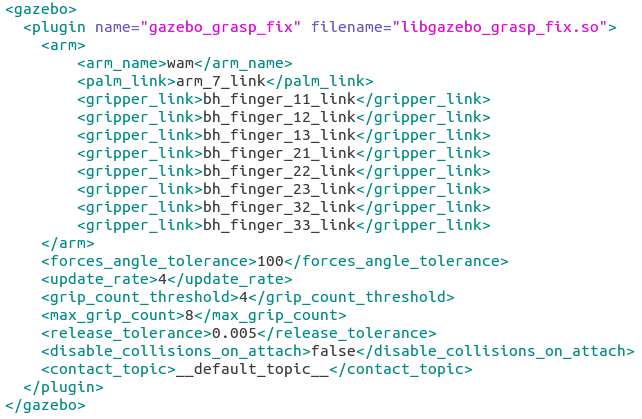
\includegraphics[width=12cm]{grasp_plugin.png}
	\caption{Implementation of the gazebo grasp plugin}
	\label{fig:graspcontrol}
\end{figure}

The AR Drone simulation package did not present any problems. The simulated drone is controlled by a ROS velocity message and is directly compatible with the \verb!tum_ardrone! package.  

To have both the AR Drone and the mobile manipulator in the same simulation
 we had to be careful with topic and frame names. The namespace `quadrotor' was used to launch the drone model and related nodes. Changing the topic names caused the simulated drone to become unstable. The  gazebo plugin in the \verb!tum_sim! package had to be modified, since it was not possible to remap the topic names related to sensor information. The simulated drone behaved in a similar way to the real drone once the correct information was being received.
 
To run the simulation of the mobile manipulator and the drone independently run the following commands on a terminal:

\begin{itemize}
	\item Mobile manipulator
	\begin{itemize}
		\item \verb!roslaunch guardian_gazebo gwam.launch!
	\end{itemize}
	\item AR Drone
	\begin{itemize}
		\item \verb!roslaunch launch_robots quadrotor_sim.launch!
	\end{itemize}
\end{itemize}

\subsection{Individual Robot Capabilities}
In order to have smart behaviours, such that the operator does not need to be concerned with basic commands, some autonomous capabilities were implemented on both robotic platforms. Mainly autonomous navigation of unknown environments for the mobile manipulator, and tracking of a given point for the drone.

\subsubsection{Mobile Manipulator}
Autonomous navigation of unknown environments was implemented with the Guardian.

The Gmapping ROS package was used to create a map of the environment as the Guardian travels through it, and to provide more robust localization within this created map. In Figure \ref{fig:gmapping} we can see an example of a map produced by Gmapping. This map and the calculated location are then used by the Navigation stack.


\begin{figure}[ht!]%
	\centering
    \subfloat[Gazebo World]{{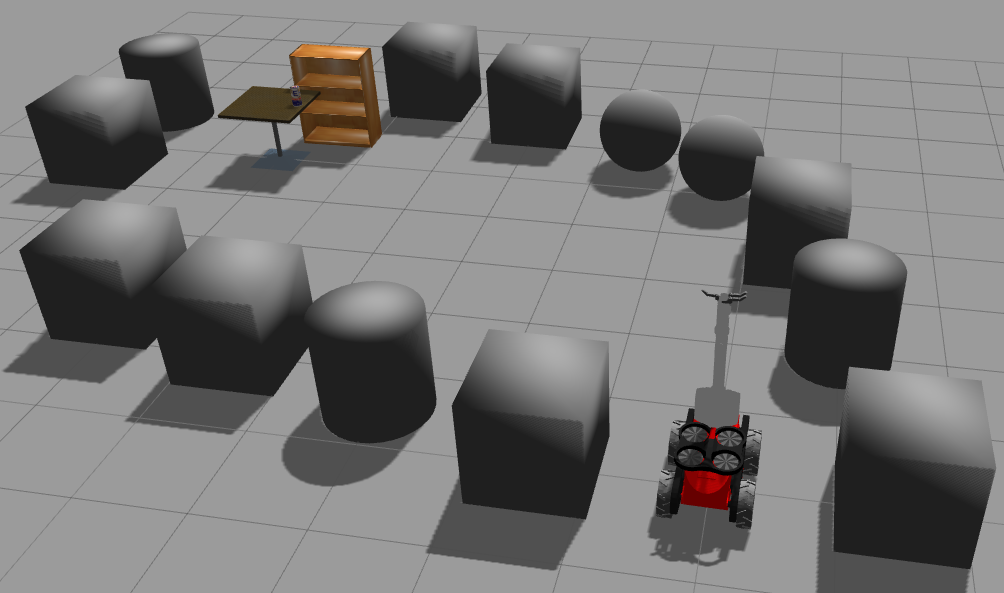
\includegraphics[height=3.8cm]{gazebo_21.png} }}  
    \qquad  
    \subfloat[Resulting Map]{{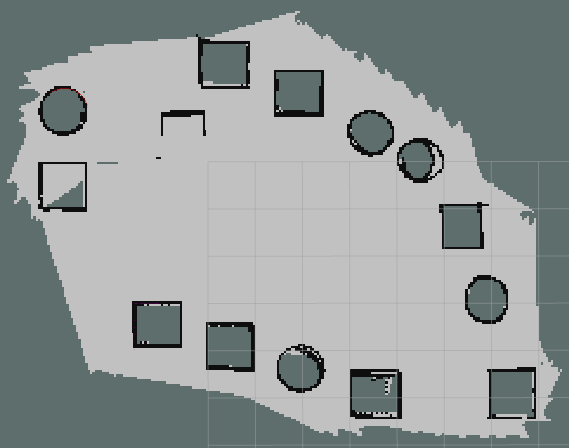
\includegraphics[height=3.8cm]{gmapping_2.png}}}
    \caption{Map produced by Gmapping}
    \label{fig:gmapping}
\end{figure}

Navigating through the environment was done through the Navigation ROS package, allowing the robot to reach a defined goal while avoiding obstacles. A special costmap plugin was used (\verb!voronoi_navigation! \footnote{https://github.com/MonicaArias/voronoi\_navigation} ), which creates a Voronoi diagram of the map given by Gmapping. This allows the system to prioritize the path with the most clearance between obstacles. We can see in Figure \ref{fig:globalPath} an example of the planned path from the starting point [x=0, y=0,  th=0] to the goal [x=4.8, y=4.4, th=1.48], a point close to the table where the can is. The path is highlighted in green, the red is the part considered by the local planner; the obstacles (in yellow) are surrounded by a buffer area where the robot might collide; and the blue lines are the Voronoi diagram where the robot tries to go on.

\begin{figure}[h!]
	\centering
    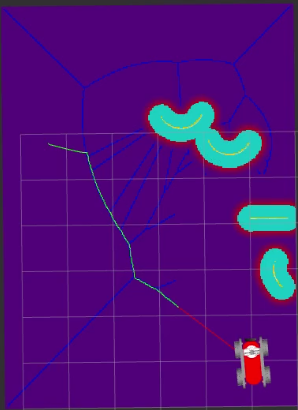
\includegraphics[width=4cm]{globalplan.png}
    \caption{Global path (in red and green) produced by the Navigation package}
    \label{fig:globalPath}
\end{figure}

One of the defined cooperative behaviours is that the drone follows the mobile base.  The extra clearance provided fullfills two roles: increased safety for the mobile base, since it is less likely to hit an obstacle when turning a corner; and it allows the drone enough space to not bump into walls. 

\vspace{10mm}

For the manipulation of a can on a table we defined 5 poses for the arm:
\begin{enumerate}
	\item Init - Arm stretched out, it is the initial pose of the arm to be able to place the quadrotor on 
		top of the Guardian
	\item Pick - Folded arm, it is the pose to grab the can
	\item Raise - Raised arm, assumes the robot is holding the can. It is the intermediary step when the drone is supposed to change point of view.
	\item Place - The arm turns to position the can on the shelf
	\item Retrieve - To move the arm from the placing position in a linear trajectory, avoiding collisions
\end{enumerate}

 These poses are shown in Figure \ref{fig:arm_poses}. They are predefined, and are only valid for our testing scenario. 

\begin{figure}[ht!]%
	\centering
    \subfloat[Init]{{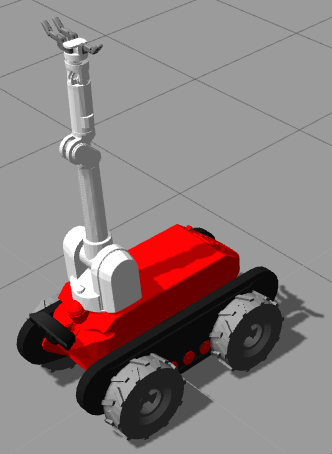
\includegraphics[height=3cm]{init_pose.png} }}  
    \qquad  
    \subfloat[Pick]{{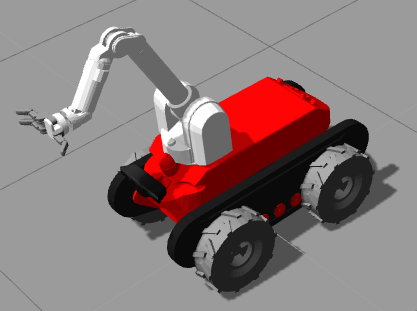
\includegraphics[height=3cm]{pick_pose.png} }}  
    \qquad  
    \subfloat[Raise]{{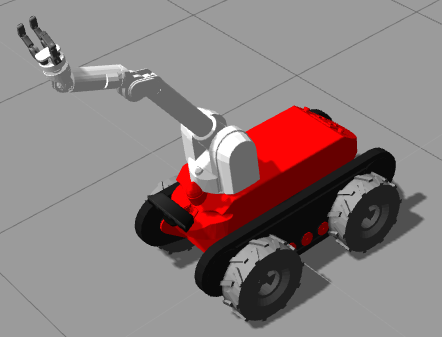
\includegraphics[height=3cm]{raise_pose.png} }}  
    \qquad  
    \subfloat[Place]{{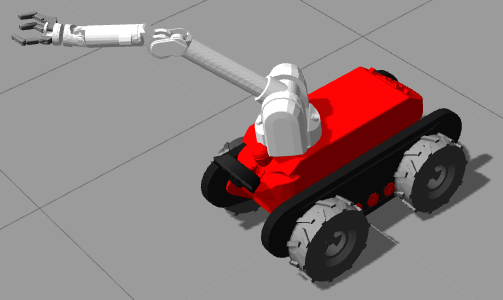
\includegraphics[height=3cm]{place_pose.png} }}       
    \qquad  
    \subfloat[Retrieve]{{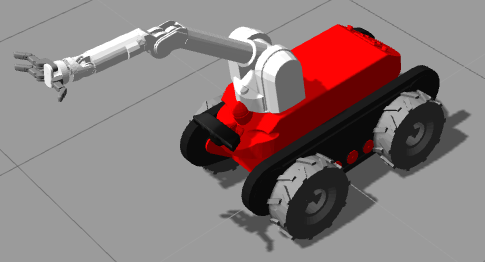
\includegraphics[height=3cm]{retrieve_pose3.png} }}       
    \caption{Arm predefined poses}
    \label{fig:arm_poses}
\end{figure}



\subsubsection{Quadrotor}
We implemented point tracking for the drone.

As explained previously, the \verb!tum_ardrone! package provides a PID controller and a position estimation, which the controller takes as the current position of the drone. On the real drone it is necessary to have various keypoints on the front camera image to avoid drifting, since PTAM is used to estimate the position.

These keypoints are not necessary in the simulation, the Extended Kalman Filter is accurate enough, only the estimated height of the drone is not very reliable, and causes the platform to drift upwards. We created an intermediary node, \textit{replace\_z}, to take in the position estimation and replace the height element with the ground truth information provided by gazebo. This proved to stabilize the drone more robustly.

Once the drone is capable to go to a commanded position we can track a reference frame. We implemented this feature with the \textit{followpoint\_drone} node. In Figure \ref{fig:posT} we can see the drone approaches the tracked frame. It is worth noting that the [x,y] coordinates of the mobile manipulator and the drone have different orientation, such that the drone is equal to the [-y,x] position of the Guardian. We took this into account for the frame tracking.

\begin{figure}[ht!]%
	\centering
    \subfloat[]{{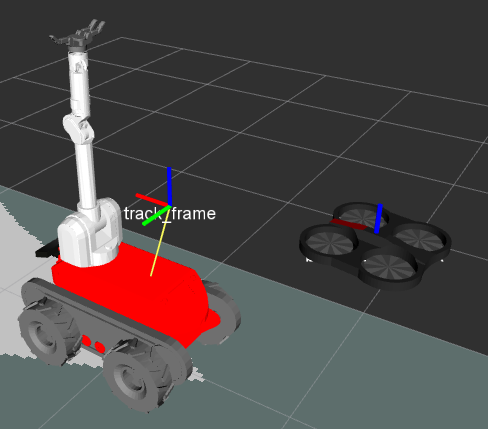
\includegraphics[height=3cm]{frame_tracking_22.png}}}  
    \qquad  
    \subfloat[]{{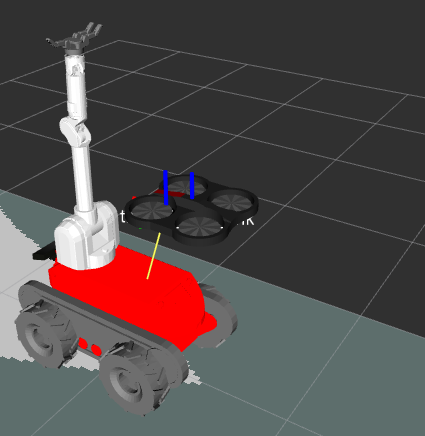
\includegraphics[height=3cm]{frame_tracking_23.png} }}  
    \caption{Position tracking}
    \label{fig:posT}
\end{figure}




\subsection{GUI programming}
Programming the GUI was facilitated by the rqt package. Setting up the interface was, however,
 a complicated task since the tutorial of rqt is not exactly finished and omitted crucial set-up details. The rqt package creates a ROS nodelet which allows access to
all the ROS useful features: subscriber, publisher, message types, etc.

Then this nodelet acts like a Qt blanc page, allowing us to program the GUI we want. It is 
important to note that the QWidgets and the ROS services run on a different thread, implying some limitations because a ROS Callback
\href{http://wiki.ros.org/rqt/Tutorials/Writing\%20a\%20C\%2B\%2B\%20Plugin}
{cannot access a Qt element}.

\begin{figure}[ht!]%
	\centering
    \subfloat[Version 1.0]{{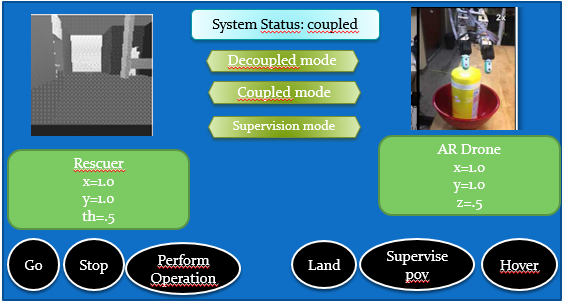
\includegraphics[width=6.5cm]{guiSketch.png} \label{fig:gui1}}}  
    \qquad  
    \subfloat[Version 2.0]{{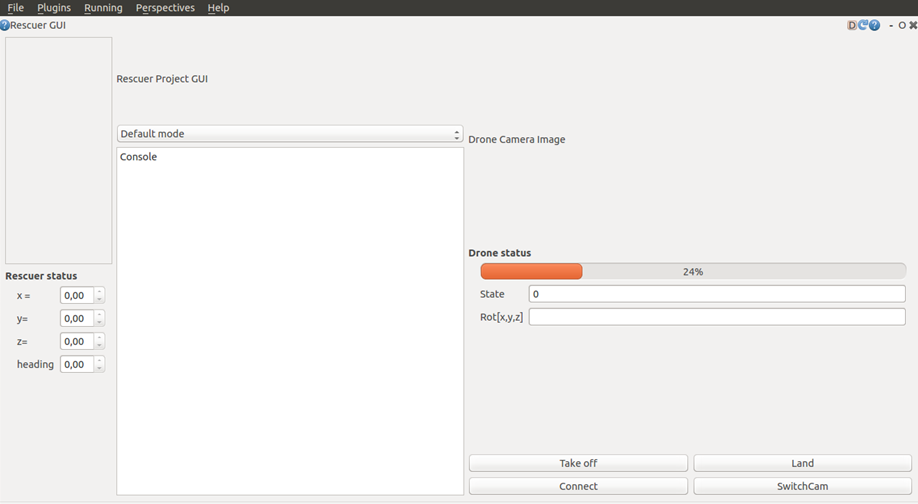
\includegraphics[width=6.5cm]{guiV2.png} }}  
    \qquad  
    \subfloat[Version 3.0]{{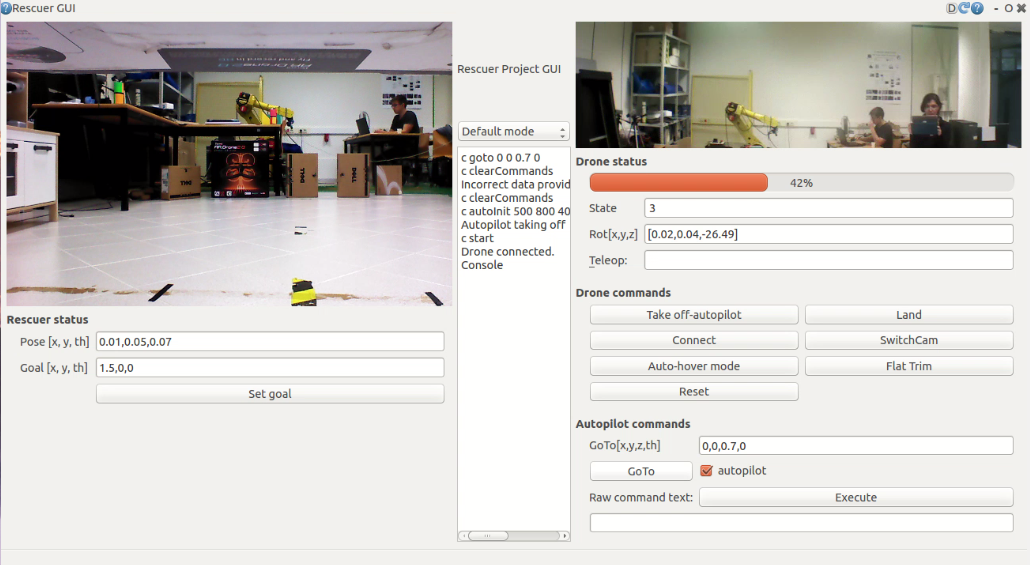
\includegraphics[width=6.5cm]{guiV3.png} \label{fig:gui3}}}       
    \caption{GUI development}
    \label{fig:gui}
\end{figure}

With the first test widget operational, the development of the GUI started based on a first sketch, shown on Figure \ref{fig:gui1}. The development of the GUI commands for the drone followed the features we were
testing on the physical robot. For the mobile manipulator the features were focused on our test scenario.

\begin{figure}[ht]
	\centering
    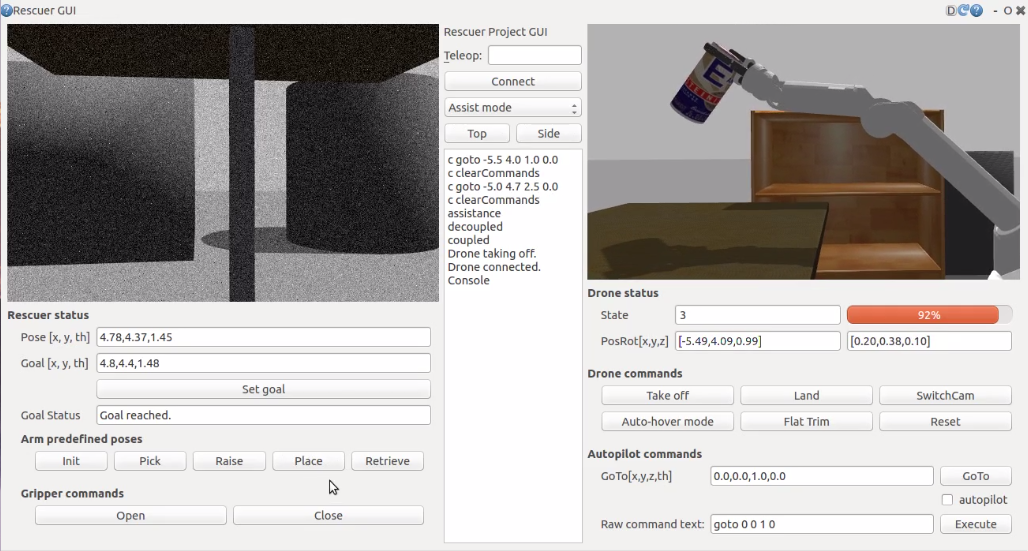
\includegraphics[width=14cm]{guiV4.png}
    \caption{Final GUI}
    \label{fig:gui4}
\end{figure}


In Figure \ref{fig:gui4} we can see the final version of the GUI. It contains the following elements:
\begin{itemize}
	\item Mobile Manipulator Control - Located on the left hand side panel
	\begin{itemize}
		\item Mobile base camera
		\item Position provided by the \textit{position\_rescuer} node, that transforms the reference frame from Gmapping into a point
		\item Goal to be sent to the Navigation package
		\item Arm poses to grab the can on the table
		\item Open and close commands for the Barret hand				
	\end{itemize}	
	\item Drone Control - Located on the right side of the panel
	\begin{itemize}		
		\item Drone camera, either bottom or front camera, can be swithced with the 'SwitchCam' button below
		\item The drone current state, with the following meaning:
		\begin{multicols}{2}
		\begin{enumerate}
			\item Unknown
			\item Initiated
			\item Landed
			\item Flying
			\item Hovering
			\item Test
			\item Taking off
			\item Landing
			\item Looping 
		\end{enumerate}
		\end{multicols}		
		\item Battery level
		\item Position read by the controller, and orientation provided by the \verb!ardrone_autonomy! 	
			driver
		\item Drone commands, including take off and landing
		\item Autopilot commands, to go to a given point with the \verb!tum_ardrone! package	
	\end{itemize}	
	\item Common commands - In the  middle of the GUI
	\begin{itemize}
		\item Tele-operation for both robots
		\begin{itemize}
			\item For the mobile base:
			\begin{itemize}
				\item "W" is forward, "X" is backwards
				\item "D" is turn right, "A" is turn left			
			\end{itemize}
			\item For the drone:
			\begin{itemize}
				\item Arrow up is forward, arrow down is backwards
				\item Arrow right is move to the right, arrow left is move to the left (there is no rotation 
				because the state estimation depends on a fixed viewpoint)
				\item Page up is upwards, page down is downwards
			\end{itemize}	
		\end{itemize}
		\item Connect button, to initialize the GUI for both robots
		\item Behaviour mode, to be able to select between decoupled, coupled and supervised (assist) modes	
		\begin{itemize}
			\item When assist mode is selected, the buttons for the possible views appear
		\end{itemize}		
		\item Console, to display information and debugging messages to the screen	
	\end{itemize}
\end{itemize}

Finally, the topics used in the GUI for communication can be seen in Figure \ref{fig:guicomm}.




\begin{figure}[ht]	
\centering
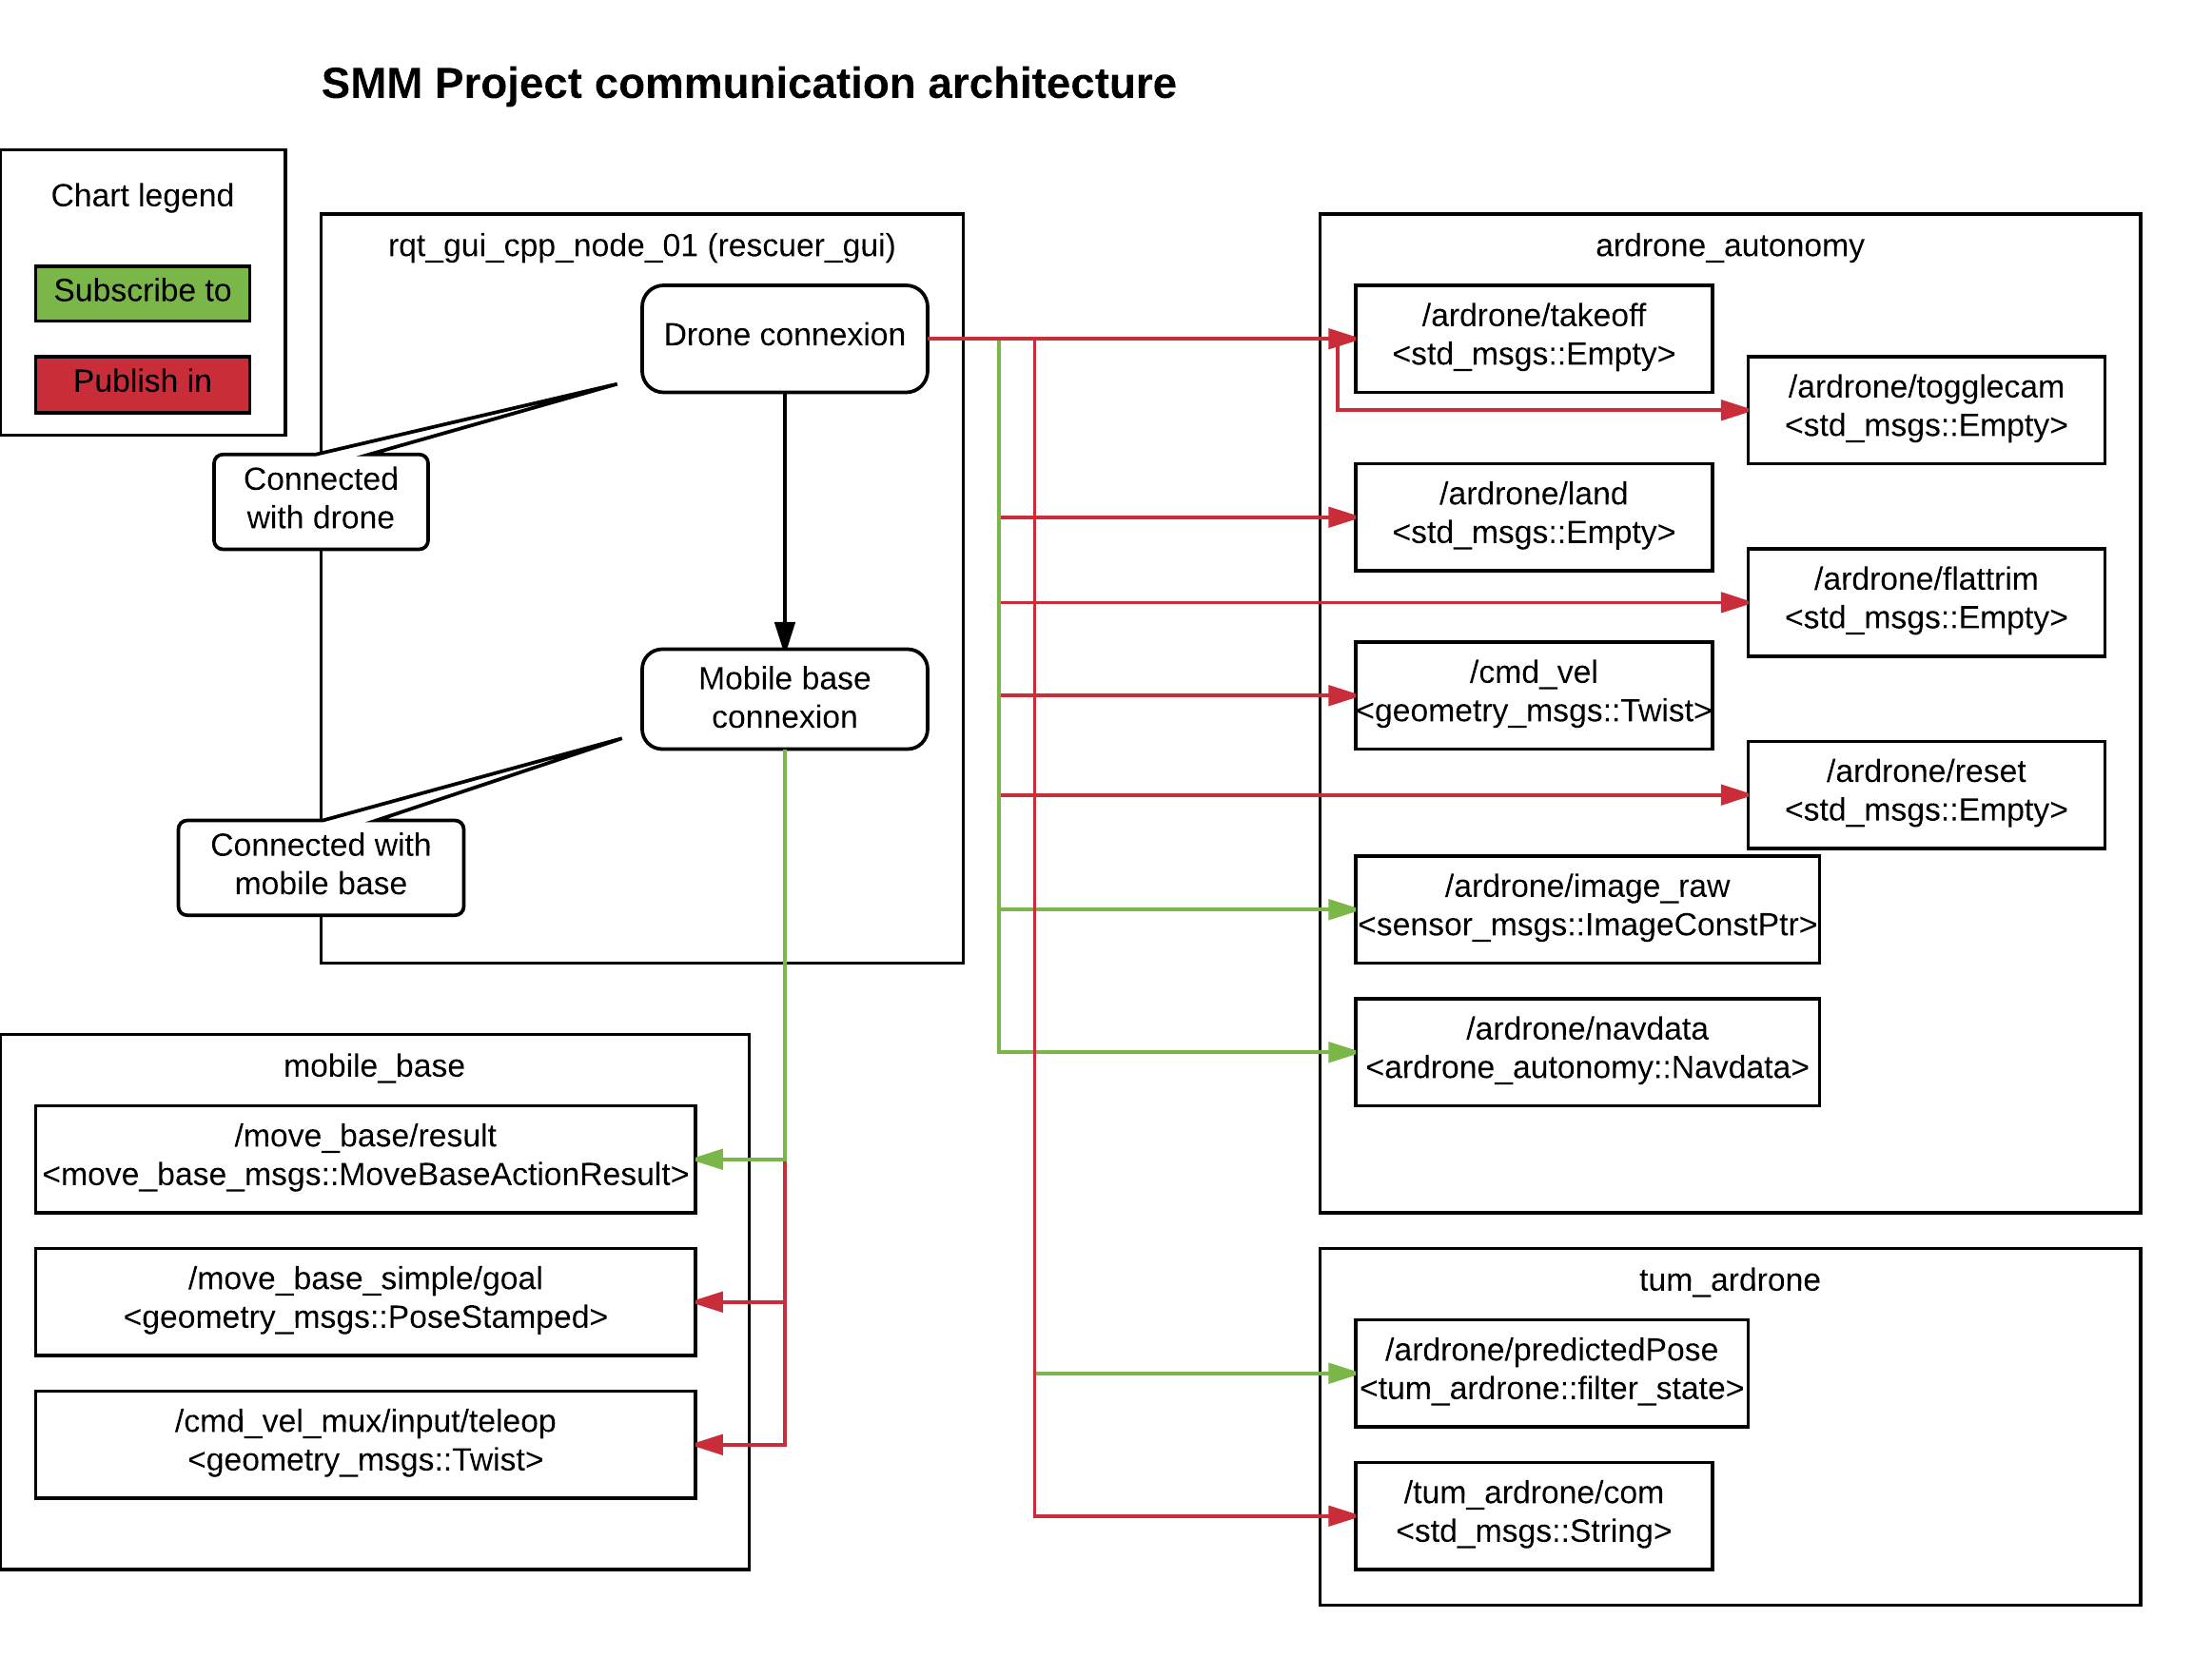
\includegraphics[width=12.7cm]{communicationArchitecture.png}
\caption{GUI Communication architecture}
\label{fig:guicomm}
\end{figure}
\clearpage


\section{Experiments and result analysis}

\subsection{Simulation testing}
The objective for our simulation scenario is to move a can from a table to a bookcase. We know the location of the table, so we can give it as a goal point to the mobile manipulator. The operator only has the developed GUI as interface to command the robots and to change behaviour mode between decoupled, coupled and supervised modes.

To run the simulation environment and the GUI we use the following commands in two terminals:
\begin{itemize}
	\item \verb!roslaunch launch_robots three_robots_sim.launch!
	\item \verb!rqt!
\end{itemize}

From the rqt window open the rescuer GUI plugin:
\begin{itemize}
   	\item Open the Plugins menu from the top of the window with Alt+P
   	\item Select Rescuer
	\item Select GUI for Rescuer
\end{itemize}


The simulation starts with the drone on top of the Guardian (Figure \ref{fig:coup1}). The initial position of the mobile manipulator is [x=0, y=0, th=0] and for the drone is [x=0, y=0, z=0.6, th=0]. The steps we followed to accomplish the task were as follows:
\begin{enumerate}

	\item \textbf{Set goal} at [x=4.8, y=4.4, th=1.48] for the mobile manipulator.
	\item \textbf{Take off} with the drone while the mobile manipulator moves towards the goal.
	\item Change to \textbf{Coupled mode}, for drone to track the mobile manipulator.
	\item Wait until the mobile manipulator reaches the goal.
	\item Change to \textbf{Decoupled mode} so the drone stops tracking the base.
	\item Change to \textbf{Assist mode}.
	\item Move the drone to \textbf{Top} view.
	\item \textbf{SwitchCam} to see from the drone's bottom camera.
	\item Put the arm in the \textbf{Pick} pose.
	\item Tele-operate the Guardian to get to a good position to grab the can.
	\item \textbf{Close} the gripper.
	\item Move arm to \textbf{Raise} pose.
	\item Move drone to provide \textbf{Side} view point.
	\item \textbf{SwitchCam} to see from the drone's front camera.
	\item Set the arm to the \textbf{Place} pose.
	\item \textbf{Open} the gripper.
	\item Move the arm to the \textbf{Retrieve} pose.
	\item Finalize by setting the arm to the \textbf{Init} pose and changing to \textbf{Decoupled mode}.
	
\end{enumerate}


In short, first we gave a goal to the mobile manipulator and used the coupled mode to have the drone follow it (steps 1 to 4). This can be visualized in Figure \ref{fig:coupledmode}. Then, in the assist mode, we used the drone's bottom camera to carefully approximate the can and grasp it (steps 6 to 11). Figure \ref{fig:assistmode1} shows the camera view of the grasping process. Finally, we observed the placing of the can from the drone's front camera, ensuring no collisions occurred (steps 12 to 17), as shown in Figure \ref{fig:assistmode2}.  

\begin{figure}[ht!]%
	\centering
    \subfloat[]{{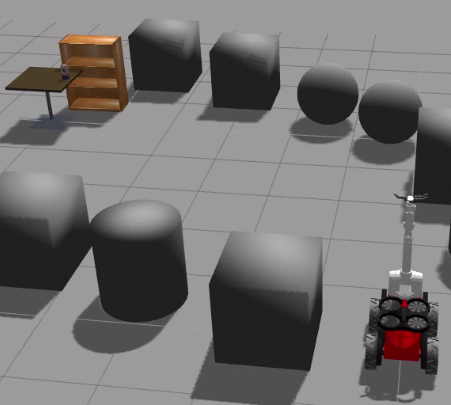
\includegraphics[height=3.9cm]{coupled_mode1.png} \label{fig:coup1}}}  
    \qquad  
    \subfloat[]{{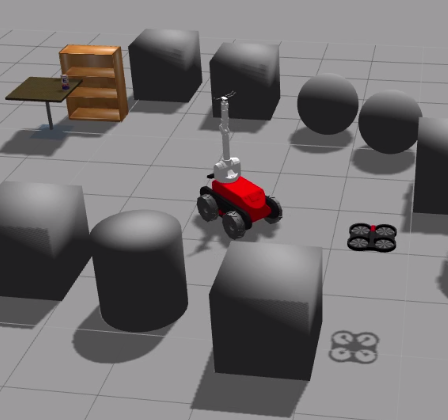
\includegraphics[height=3.9cm]{coupled_mode2.png} }}  
    \qquad  
    \subfloat[]{{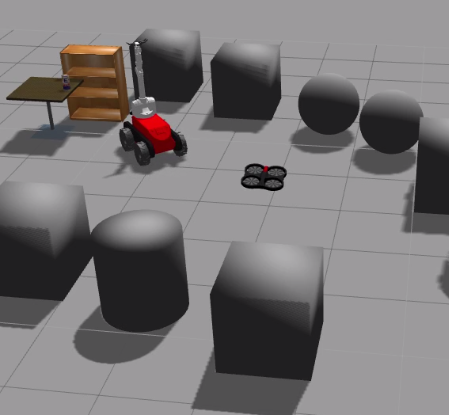
\includegraphics[height=3.9cm]{coupled_mode3.png}}}   
    \qquad  
    \subfloat[]{{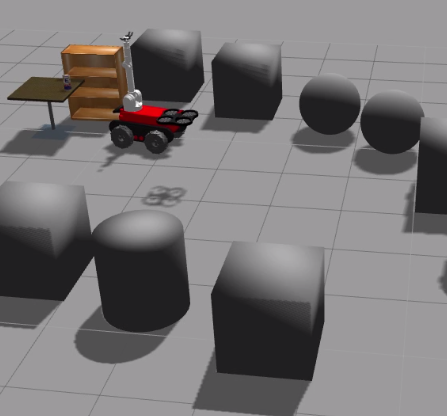
\includegraphics[height=3.9cm]{coupled_mode4.png} }}  
    \qquad  
    \subfloat[]{{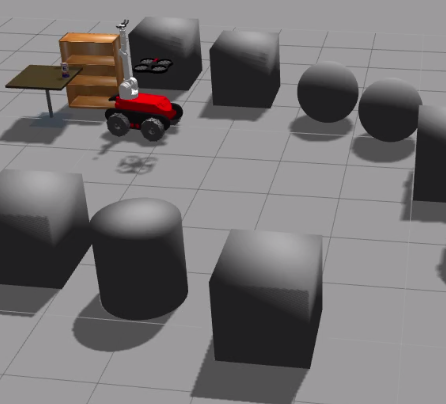
\includegraphics[height=3.9cm]{coupled_mode6.png} \label{fig:coup5}}}      
    \caption{Coupled mode to reach a goal}
    \label{fig:coupledmode}
\end{figure}

\begin{figure}[ht!]%
	\centering
    \subfloat[]{{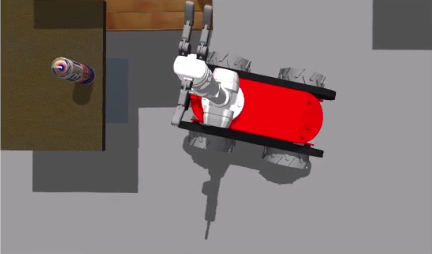
\includegraphics[height=3cm]{assist_mode1.png} \label{fig:assist1}}}  
    \qquad  
    \subfloat[]{{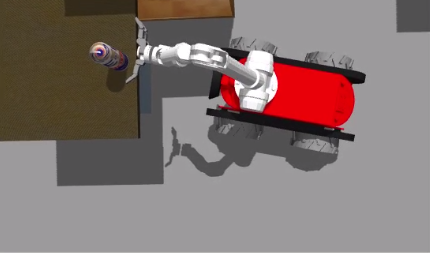
\includegraphics[height=3cm]{assist_mode2.png} }}  
    \qquad  
    \subfloat[]{{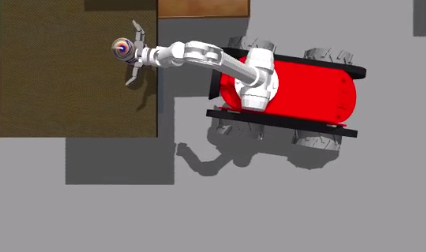
\includegraphics[height=3cm]{assist_mode3.png}}}   
    \qquad  
    \subfloat[]{{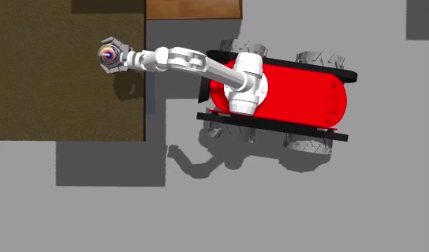
\includegraphics[height=3cm]{assist_mode4.png} }}     
    \caption{Drone's bottom camera view in assist mode}
    \label{fig:assistmode1}
\end{figure}

\begin{figure}[ht!]%
	\centering
    \subfloat[]{{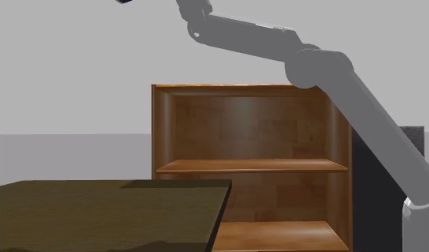
\includegraphics[height=3cm]{assist_mode5.png}}}  
    \qquad  
    \subfloat[]{{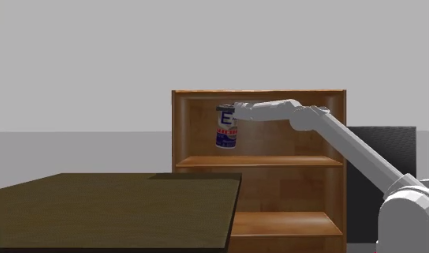
\includegraphics[height=3cm]{assist_mode6.png} }}  
    \qquad  
    \subfloat[]{{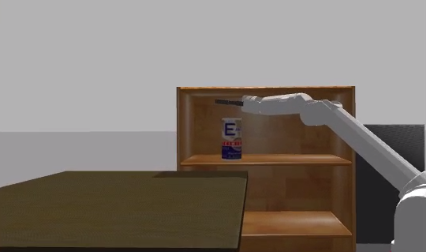
\includegraphics[height=3cm]{assist_mode7.png} }}  
    \qquad  
    \subfloat[]{{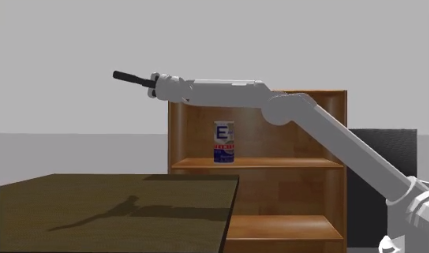
\includegraphics[height=3cm]{assist_mode8.png} }}      
    \caption{Drone's front view in assist mode}
    \label{fig:assistmode2}
\end{figure}


We found the view provided by the drone was enough to fine tune the picking and placing positions of the can. On the other hand, the specific view points used for this test were highly constrained by the drone's controller, since it does not rotate. A better controller would allow us to gain more knowledge about the scene and it would give more options to supervise from, for instance rotating around the object might be a better option than a view from above if the ceiling is too low. 



\subsection{Improvement and future work}
\subsubsection{Graphical user interface}
Full control of a mobile manipulator and of a drone requires a lot of different commands. On the presented GUI we had the physical drone to run tests on, which caused the amount of available commands to increase. A good improvement can be done by adding different tabs that focus on one robot, such that there is the general view for some commands, like take off and landing, but a different tab for things like flat trim,  which is useful to stabilize the drone. 

Additional features should be included in the GUI. As stated before, the current arm poses only work with our specific testing scenario, since they were used for demonstration purposes. It is needed to add Cartesian control to the arm, to be able to operate it smoothly from the keyboard. 
Ideally, the grasping procedure would be automatized by integrating the view from the drone with a motion planner. In this way the operator would have to make sure the drone has a good view of the object and the gripper, and the system would try to grasp the object autonomously.

Since our approach is in between human operated and autonomous behaviour, it would be useful to implement an alarm system to notify the user when a robot might fail an autonomous operation. In this way, the operator could take over the task in a timely manner. In the current system the operator can take over, but attention at all times is needed and there is not a clear way of cancelling current objectives (like reaching a  goal for the Guardian).

In general, more scenarios need to be tested to prove the reliability of the system. Different users need to perform the given task to improve the design of the GUI and make it more intuitive.

\subsubsection{Cooperative behaviour}

We implemented following the mobile manipulator with the drone, and providing different view points for manipulation. 
We need to add obstacle avoidance capabilities to the drone when it is tracking the Guardian. It would also be interesting to add visual tracking, since position tracking leaves the drone considerably behind.
A controller has to be built for the drone to improve the different views, since the one we are using does  not allow it to rotate.  

The other behaviours suggested for the supervisor mode also have to be implemented: scouting ahead of the mobile manipulator and moving in a restricted semi-circle to gain more awareness of the environment.


\subsubsection{Simulation}
The performance of the mobile manipulator and the drone have to be verified with the real robots. For instance the drone is very stable in the simulated world, and we believe a more detailed AR Drone model would help to test stability and control issues of the real platform.
The Guardian model also needs to be revised, since the rotational motion is not smooth.


\clearpage
\section{Conclusion}
Cooperative robotics is the next step of evolution in robotic systems.
Their versatility and relative architectural simplicity make them both very useful while
keeping a design simple enough to be maintainable.

The general lack of GUI in robotic systems is also a problem that have to be addressed. 
Robot programmers generally focus on software and middle-ware accurate programs while 
overlooking the final user activities which might be greatly facilitated by a clear and 
well-designed GUI.
By using both good middle-ware libraries (like ROS) combined with good higher level
software (as Qt) programs for robots can get both easier to use and provide a better 
feedback.

Implementing cooperative behaviours into semi tele-operated multi-robots system allows to release 
the operator task load. This permit to focus on the end-goal of the mission while not dealing 
with situational issues such as camera positioning or sensor feedback accuracy.

\bibliography{bib}
\bibliographystyle{abbrv}
\listoffigures
\end{document}

\end{document}